\documentclass[11pt,UTF8]{ctexart}
\title{低粘性流体中间夹高粘性库埃特流体}
\author{马坤}
\date{2019.10.16}
\usepackage{amsmath}
\usepackage{graphicx}
\usepackage{caption}
\usepackage{subcaption}
\usepackage[left=1in, right=1in, top=1in, bottom=1in]{geometry}
\begin{document}
    \maketitle
    \par{本实验选用的二维库埃特流作为模拟的对象,选取$U_0=0.1$
    作为上固体板的速度,下固体板速度为0。模拟的范围为$H=L=1$的
    矩形区域,流体密度均是$\rho_0=1$,由于是库埃特流,所以有其
    对应的控制方程与解,形式如下:
    $$
    \frac{\partial p}{\partial x}=\frac{\partial}{\partial y}(\eta\frac{\partial u}{\partial y}).\eqno(1)
    $$$$
    u = U_0\frac{y}{H}.\eqno(2)
    $$
    库埃特流本来是没有压强差的,也就是$(1)$中$\frac{\partial p}{\partial x}=0$。
    但是我们此次的模拟流体的粘性系数会发生变化所以,其压强差不可能为0,于是这里的
    控制方程形式就与泊肃叶流一致。
    }
    \par{低粘性流体中间夹高粘性流体,我们采用示性函数$\phi$来
    表示,其定义如下:
    $$
    \phi =
    \begin{cases}
        \frac{1}{2}[\tanh{\frac{y-H/3}{W}}+1],\text{y$\leq$H/2}\\
        \frac{1}{2}[-\tanh{\frac{y-2H/3}{W}}+1],\text{y$>$H/2}
    \end{cases}
    $$
    在大粘性流体中为1,在小粘性流体中为0,在边界
    $(y=H/3,y=2H/3)$上为0.5。数值模拟中,我们分别选取了
    $W=1,W=0.1$的情况。利用$\phi$可以定义流体各处的粘性系数:
    $$\eta = 1+\frac{\eta_s}{\eta_l}\phi-\phi.\eqno(3)$$
    模拟中我们均采取了高低粘性系数流体的粘性比为
    $rate=\frac{\eta_s}{\eta_l}=1000$,并取
    $Re=10000$使得粘性系数最大值与黄老师的数值匹配。}
    \par{类似的这里的流体中力和压强梯度有一个替代的关系:
    $F = -\frac{\partial p}{\partial x}$,于是我们将$(2)(3)$
    代入$(1)$就可以计算得到力的表达式:
    $$
    F =
    \begin{cases}
        U_0\frac{rate-1}{2W}[1-\tanh^2{\frac{y-H/3}{W}}]/H,\text{y$\leq$H/2}\\
        -U_0\frac{rate-1}{2W}[1-\tanh^2{\frac{y-2H/3}{W}}]/H,\text{y$>$H/2}
    \end{cases}
    $$}
    \par{数值模拟中,我们将区域$[0,1]\times[0,1]$划分为了
    $200\times 200$个网格点。也即是网格间距为$\triangle x
    =\frac{1}{199}$,时间步长取为$\triangle t=0.03
    \triangle x=\frac{0.1}{199}$.图1为$W=1$算到两时间步
    之间的误差小于$10^{-6}$的图片。图2为$W=0.1$算到达到最大
    时间$(maxtime=200)$停机的图片
    }
    \begin{figure}[h]
        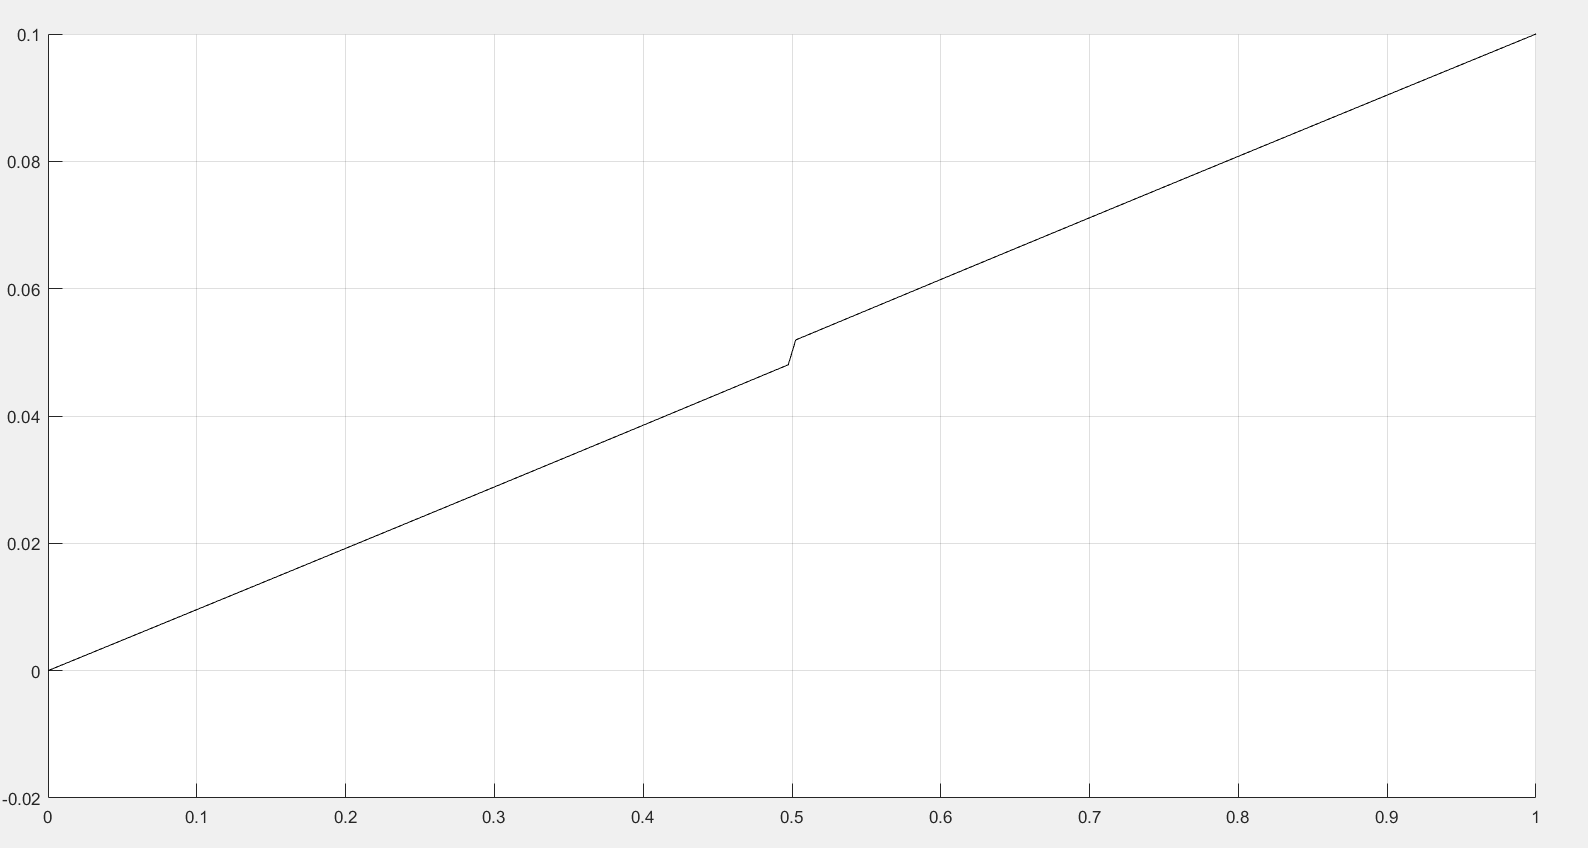
\includegraphics[width=\textwidth]{W=1.png}
        \caption{$W=1$的图像}
    \end{figure}
    \begin{figure}[h]
        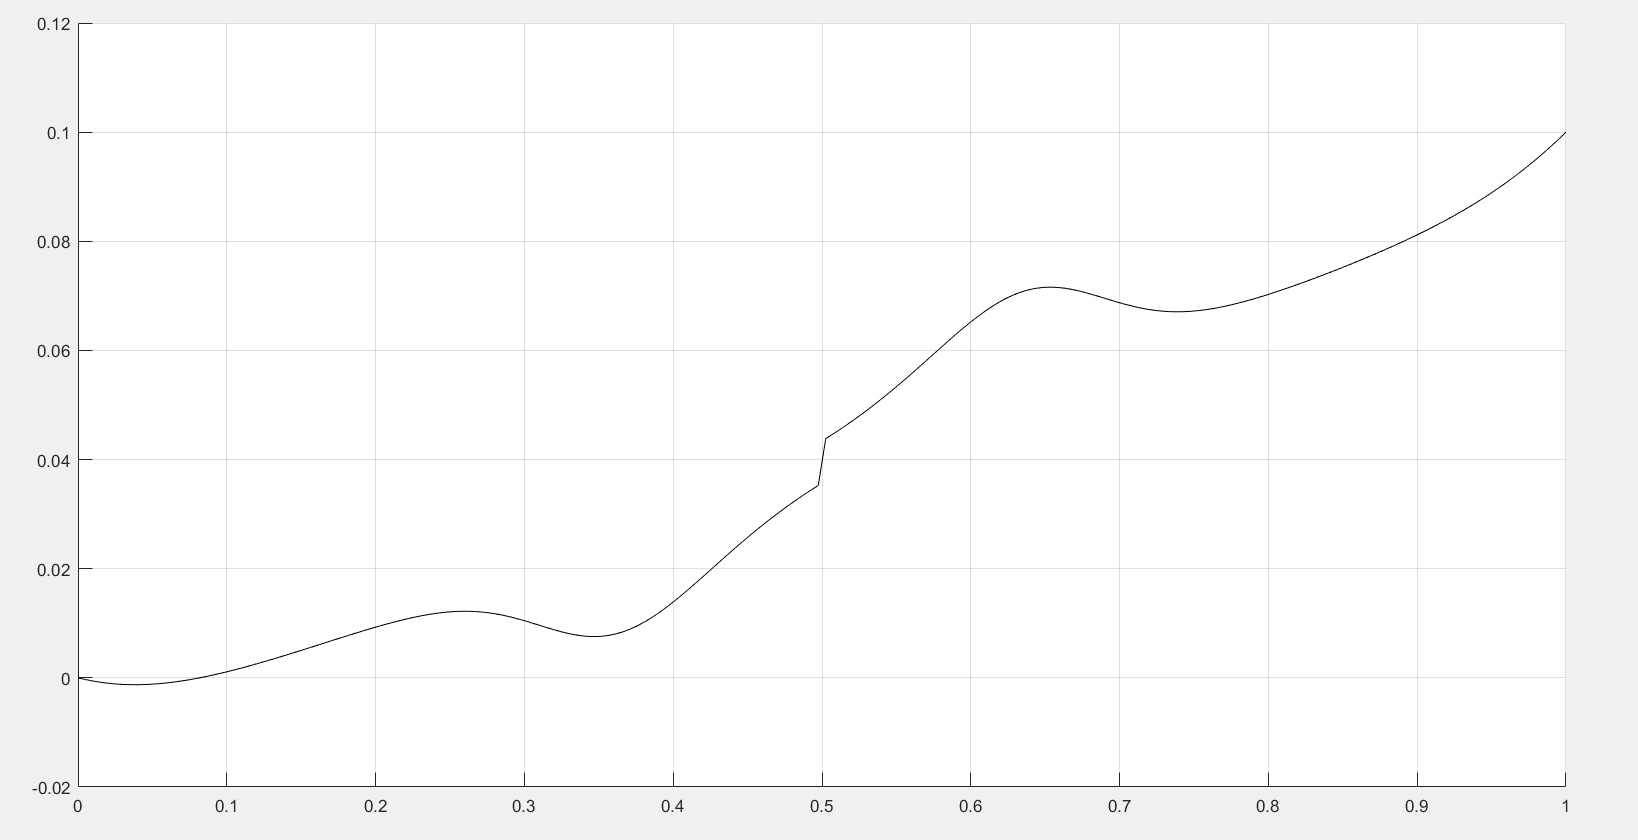
\includegraphics[width=\textwidth]{W=01.png}
        \caption{$W=0.1$的图像}
    \end{figure}
\end{document}